\documentclass{article}
\usepackage{ amssymb }
\usepackage{amsmath}
\usepackage{mathtools}
\usepackage{tikz}
\usepackage{multicol}
\usepackage{float}
\usepackage{graphicx}
\usepackage{subcaption}
\usepackage{hyperref}
\usepackage[super]{nth}
\usepackage[margin=0.8in]{geometry}

\title{Numerical methods for Differential equations Report 1}
\author{Malte Wegener (4672194)}
\date{October 2019}

\begin{document}

\maketitle
    
\section{Maxima of  2 Dimensional functions}

A sufficiently smooth function $f(x)$ has a local maximum in $x_{0}$ if there exits $\delta > 0$ such that $f(x) \leq f(x_{0})$ for all $x, \mid x - x_{0} \mid > \delta$ \par
Therefore $f(x_{0}+\delta)-f(x_{0}) \leq 0$ for sufficiently small $\delta$.
If we divide this by a small positive $\delta$, we get $\frac{f(x_{0}+\delta)-f(x_{0})}{\delta}\leq 0$.
Taking the limit as $\delta$ goes to 0, we get
\begin{equation}
   \lim_{\delta\to 0^{+}} \frac{f(x_{0}+\delta)-f(x_{0})}{\delta}\leq 0
\end{equation}

\begin{equation}
   f'(x_{0})\leq 0
\end{equation}

Similarly for $\delta < 0$

\begin{equation}
   \lim_{\delta\to 0^{-}} \frac{f(x_{0}+\delta)-f(x_{0})}{\delta}\geq 0
  \end{equation}
   
\begin{equation}
   f'(x_{0})\geq 0
\end{equation}

Thus $f'(x_{0}) = 0$

In order to separate maxima from minima and saddle points, the second derivative has to be analysed.
Let $f(x)$ be a function with a maximum in $x=x_{0}$ that can be expanded by a taylor series around $x_{0}$. f in the neighbourhood of $x_{0}$ can than be described by the following Taylor series.
\begin{equation}
    f(x_{0}+\delta) = f(x_{0})+\delta*f'(x_{0})+\frac{\delta^2}{2}*f''(x_{0}) + \mathcal{O}(\delta^3)
\end{equation}
As $f'(x_{0}) = 0$, as proven in a), This series can be rearranged for $f''(x_{0})$.

\begin{equation}
    f(x_{0}+\delta) - f(x_{0}) = \frac{\delta^2}{2}*f''(x_{0}) + \mathcal{O}(\delta^3)
\end{equation}
 As $f(x_{0}+\delta) - f(x_{0}) \leq 0$ in the neigborhood of $x_{0}$.
\begin{equation}
    0 \geq \frac{\delta^2}{2}*f''(x_{0}) + \mathcal{O}(\delta^3)
\end{equation}

Dividing by $\frac{\delta^2}{2}$.

\begin{equation}
    0 \geq f''(x_{0}) + \mathcal{O}(\delta)
\end{equation}

\begin{equation}
    0 \geq \lim_{\delta \to 0} f''(x_{0}) + \mathcal{O}(\delta)
\end{equation}

\begin{equation}
    0 \geq f''(x_{0})
    \label{eq:proooof}
\end{equation}

The derivative of a 2 dimensional function can be expressed as a vector pointing in the direction of the steepest direction uphill.
Let u be a be a sufficiently smooth function with a maximum in $ \left<x_{0}, y_{0}\right> $. $ u: \mathbb{R}^{2} \to \mathbb{R} $.
Let $f1(x) = u(x,y=y_{0})$ and $f2(y) = u(x=x_{0},y)$. Then
\begin{equation}
    \frac{d}{dx}f1(x)\bigg|_{x=x_{0}} = 0 = \frac{\partial}{\partial x}f1(x)\bigg|_{x=x_{0},y=y_{0}}
\end{equation}{}
\begin{equation}
    \frac{d}{dy}f2(y)\bigg|_{y=y_{0}} = 0 = \frac{\partial}{\partial y}f2(y)\bigg|_{x=x_{0},y=y_{0}}
\end{equation}{}

Thus $\nabla u = \mathbf{0}$

Similarly to the 1D case, the second derivative has to be analyzed. For this purposes the second derivative is defined as the Hessian of the function.
First the quadratic form of the Hessian is analyzed. Let $H$ be the Hessian matrix and $\mathbf{v}=\langle p, q\rangle$ a unit vector.
\begin{equation}
 H = \begin{bmatrix}
      \frac{\partial^2 u}{\partial x^2} & \frac{\partial^2 u}{\partial xy}\\
      \frac{\partial^2 u}{\partial xy} & \frac{\partial^2 u}{\partial y^2}\\
    \end{bmatrix}
\end{equation}

\begin{equation}
\mathbf{v}^{T} H \mathbf{v}= p^2\frac{\partial^2 u}{\partial x^2}+(p+q)\frac{\partial^2 u}{\partial xy} +q^2\frac{\partial^2 u}{\partial x^2}
\end{equation}

\begin{align*}
D_{\mathbf{v}}\left(D_{\mathbf{v}} u\right)=\mathbf{v}\cdot \nabla(\mathbf{v} \cdot \nabla u)=\mathbf{v}\cdot \nabla(p\frac{\partial u}{\partial x}+q\frac{\partial u}{\partial y})\\
D_{\mathbf{v}}\left(D_{\mathbf{v}} u\right)=p^2\frac{\partial^2 u}{\partial x^2}+(p+q)\frac{\partial^2 u}{\partial xy} +q^2\frac{\partial^2 u}{\partial x^2}
\end{align*}

Thus 
\begin{equation}
\mathbf{v}^{T} H \mathbf{v}=D_{\mathbf{v}}\left(D_{\mathbf{v}} u\right)
\end{equation}


Every plane passing through the maximum of $u$ in a direction of $\mathbf{v}$ has a single variable function in the intersection with $u$, which also has a maximum in the maximum of $u$. Thus its second derivative is $D_{\mathbf{v}}\left(D_{\mathbf{v}} u\right)$.
As $D_{\mathbf{v}}\left(D_{\mathbf{v}} u\right) \leq 0   \forall \mathbf{v}$, as proven in \autoref{eq:proooof}. As $\mathbf{v}^{T} H \mathbf{v}=D_{\mathbf{v}}\left(D_{\mathbf{v}} u\right)$, the Hessian of $u$ is semi negative definite.


\newpage
\section{Properties of the 1D negative Laplacian}
A domain $\Omega=\left[0,1\right]$ that is descretized as a uniform grid $\Omega_h$ with a uniform stepsize $h$, has $1/h+1$ grid points if 1 is an integer multiple of $h$. If it is not, however the last point of $\Omega_h$ is not on the boundary.
\begin{figure}[H]
\centering
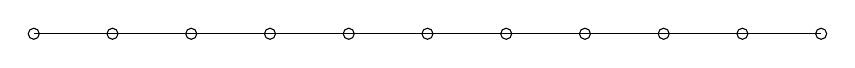
\begin{tikzpicture}
    \foreach \x in {0,...,10} 
        \draw (\x,3) circle (2pt);
    \draw (0,3) -- (10,3);
\end{tikzpicture}
\caption{$\Omega_h$}
\end{figure}

Let $\mathcal{L}=-\frac{d^{2}}{d x^{2}}$. Let u be discrete on a grid with a stepsize of $h$.
\begin{align}
    u_i &= u_i\\
    u_{i+1} &= u_i + h * u_i' + h^2/2 * u_i'' + h^3/6 * u_i''' + \mathcal{O}\left(h^4\right)\\
    u_{i-1} &= u_i - h * u_i' + h^2/2 * u_i'' - h^3/6 * u_i''' + \mathcal{O}\left(h^4\right)\\
\end{align}
\begin{align}
    D_x^+ &= \frac{u_{i+1}-u_i}{h} = u_i' + h/2 * u_i'' + h^2/6 * u_i''' + \mathcal{O}\left(h^3\right)\\
    D_x^- &= \frac{u_{i+1}-u_i}{h} = u_i' - h/2 * u_i'' + h^2/6 * u_i''' + \mathcal{O}\left(h^3\right)\\
    D_{xx} &= -1/h*\left(D_x^+ - D_x^-\right) = u_i'' + \mathcal{O}\left(h^2\right)\\
\end{align}
\begin{equation}
    \mathcal{L} \approx \frac{-u_{i-1}+2u_i-u_{i+1}}{h^2}
\end{equation}
This can be assembled in to a tridiagonal matrix $A$.
\begin{figure}[H]
    \centering
    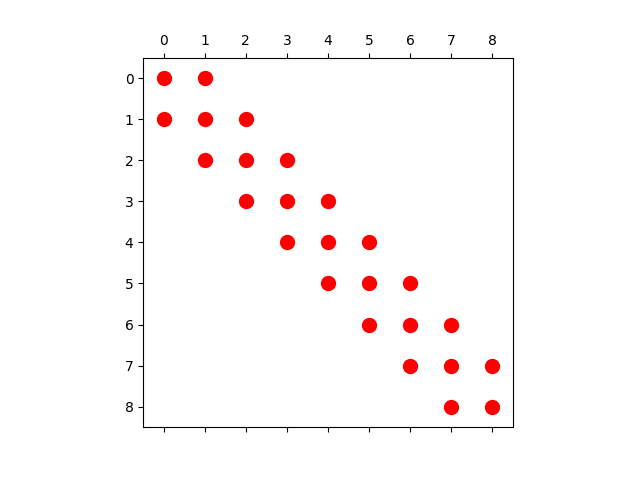
\includegraphics[width=.8\linewidth]{2spy.png}
    \caption{Structure of the Matrix $A$}
\end{figure}
As this matrix is small in size, the eigenvalues can be calculated numerically, as well as analytically. These eigenvalues can be compared to the first 9 eigenvalues of the Laplacian. It can be seen that the eigenvalues are very similar in the first eigenvalues but deviate significantly for later eigenvalues. Furthermore it can be seen that the eigenvalues are purely real.
\begin{figure}[H]
    \centering
    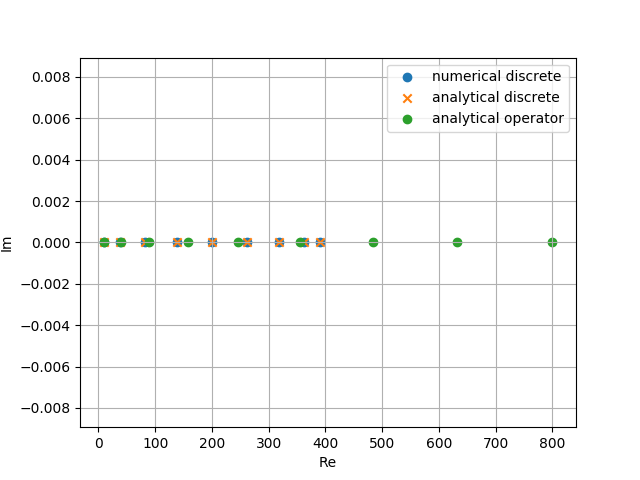
\includegraphics[width=.9\linewidth]{eigenvals.png}
    \caption{Eigenvalues of $A$ and $\mathcal{L}$}
\end{figure}
The corresponding eigenvectors can be plotted on the on the inner points of the domain together with the eigenfunctions of the Laplacian. This shows, that the eigenvectors are the eigenfunctions sampled on every grid point.
\begin{figure}[H]
    \centering
    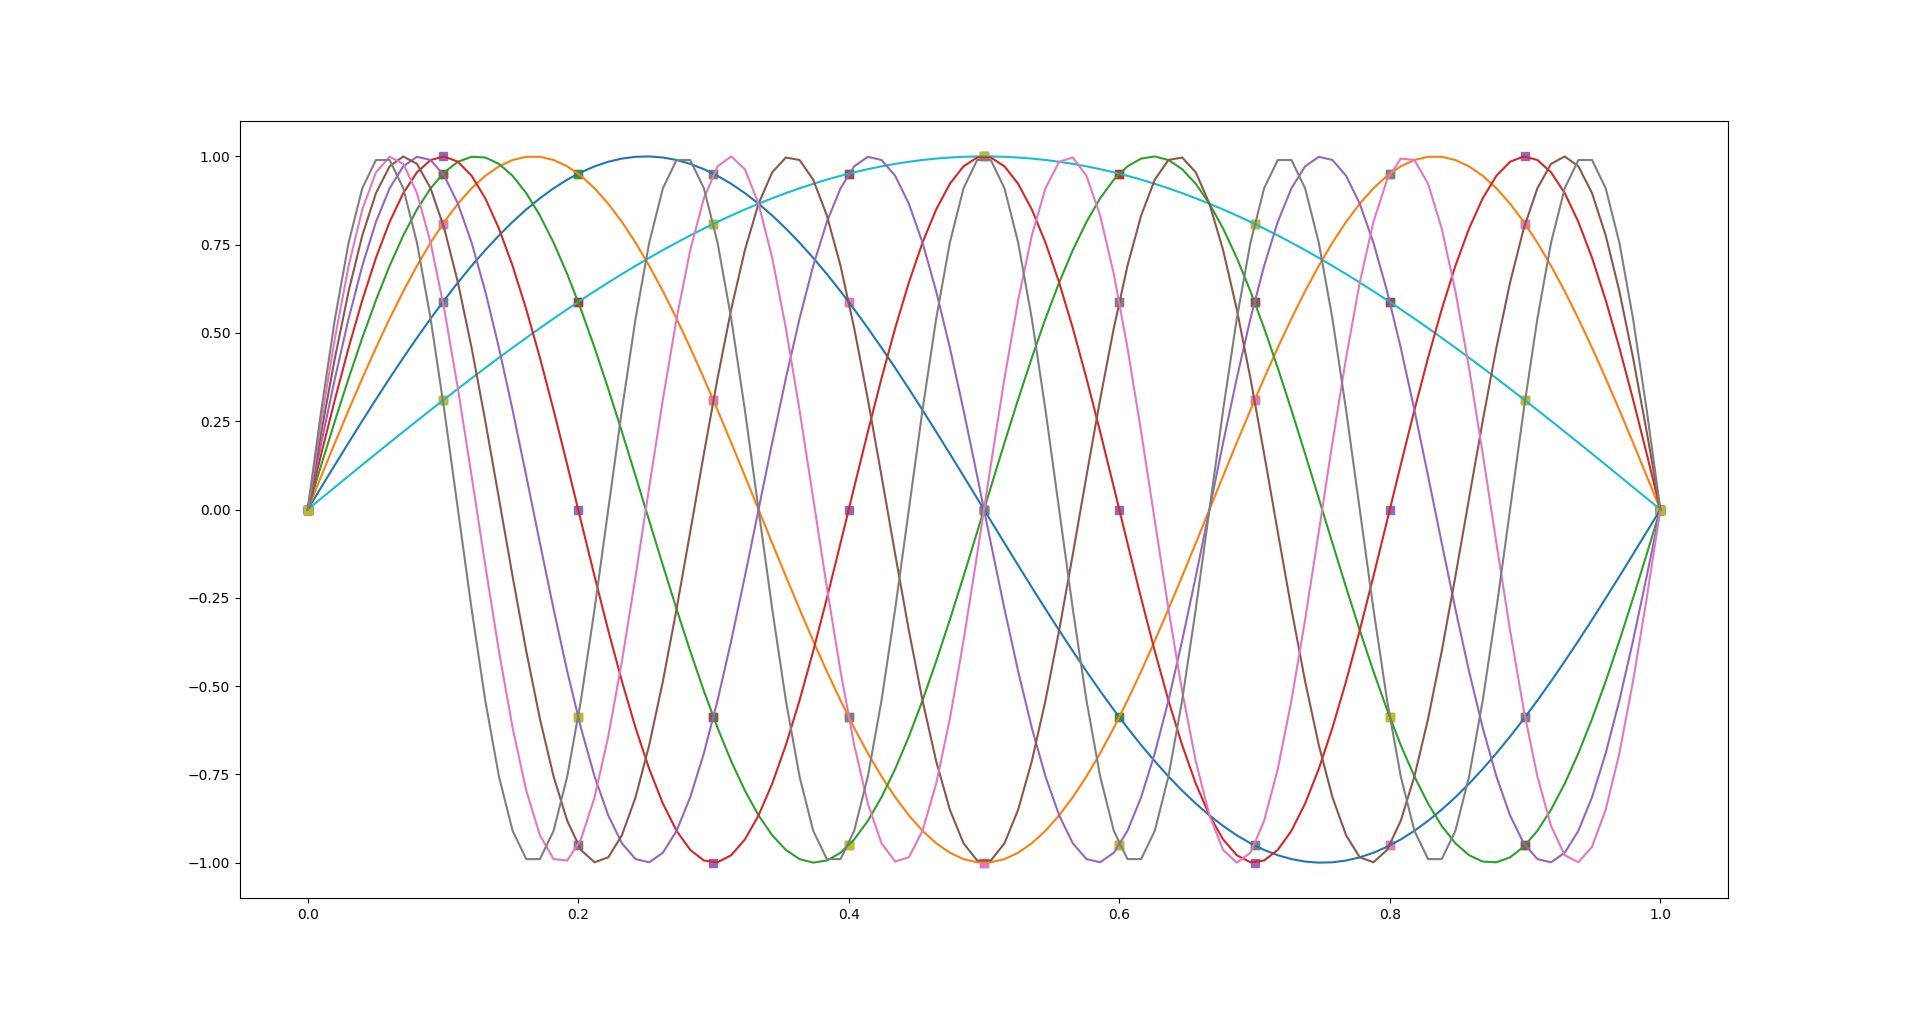
\includegraphics[width=.9\linewidth]{Eigenfuncs.png}
    \caption{Discrete eigenvectors (+) and continuous eigenfunctions}
\end{figure}

Plotting the \nth{10} Pair of eigenvector and eigenfunction, it can be seen that the eigenvector only samples the eigenfunction in its roots.  This pair is therefore the first one that can not be resolved on the chosen grid.

\begin{figure}[H]
	\centering
	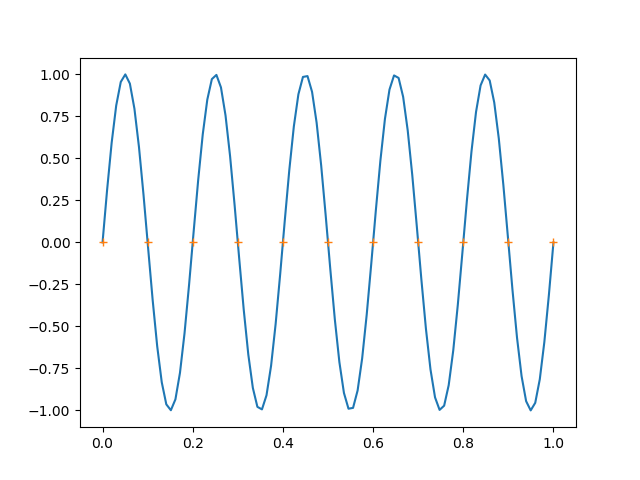
\includegraphics[width=.9\linewidth]{1thpair.png}
	\caption{\nth{10} Pair of eigenvector and eigenfunction}
\end{figure}

\section{1D boundary value problem}
Considering the following Boundary value problem, the solution can be found analytically.

\begin{align}
    -\frac{d^{2} u}{d x^{2}}=f_{i}, & x \in(0,1) \\ u(0)=1, & u(1)=2 \\ f_{1}(x)=1, \quad f_{2}(x)=e^{x}, & x \in[0,1]
\end{align}

\begin{align}
    -\frac{d^{2} u_1}{d x^{2}}=1 \\
    - d^2 u_1 = dx^2 \\
    - d u_1 = (x+C_1) dx\\
    - u_1 = \frac{1}{2}x^2 + C_1 x + C_2\\
    \text{with} u(0)=1,  u(1)=2 \\
    u_1 = -\frac{1}{2}x^2 - \frac{1}{2} x - 1\\
\end{align}

\begin{align}
    -\frac{d^{2} u_2}{d x^{2}}=e^x \\
    -d^2 u_2 = e^x dx^2 \\
    -d u_2 = (e^x+C_1) dx\\
    u_2 = -e^x + C_1 x + C_2\\
    \text{with} u(0)=1,  u(1)=2 \\
    u_2 = -e^x + e x + 2\\
\end{align}

\subsection{Symetrical Domain}
In order to solve the given problem the second derivate has to be discretized on a grid with a stepsize of h.

\begin{figure}[H]
    \centering
    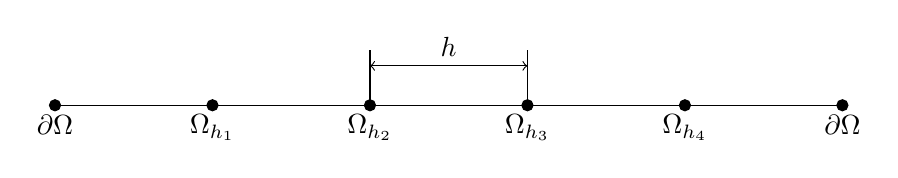
\begin{tikzpicture}
        \foreach \x in {1,...,4} 
            \filldraw (2*\x,5) circle (2pt);

        \filldraw (10,5) circle (2pt);
        \filldraw (0,5) circle (2pt);
        \draw (0,5) node[anchor=north] {$\partial \Omega$};
	  \draw (2,5) node[anchor=north] {$\Omega_{h_1}$};
	  \draw (4,5) node[anchor=north] {$\Omega_{h_2}$};
	  \draw (6,5) node[anchor=north] {$\Omega_{h_3}$};
        \draw (8,5) node[anchor=north] {$\Omega_{h_4}$};	
        \draw (10,5) node[anchor=north] {$\partial \Omega$};
        \draw (0,5) -- (10,5);
        
       \draw[arrows=<->](4,5.5) -- (6,5.5);
       \draw (4,5) -- (4,5.7);
       \draw (6,5) -- (6,5.7);
       \draw (5,5.5) node[anchor=south] {$h$};
    \end{tikzpicture}
\end{figure}

\begin{align}
    u_i &= u_i\\
    u_{i+1} &= u_i + h * u_i' + h^2/2 * u_i'' + h^3/6 * u_i''' + \mathcal{O}\left(h^4\right)\\
    u_{i-1} &= u_i - h * u_i' + h^2/2 * u_i'' - h^3/6 * u_i''' + \mathcal{O}\left(h^4\right)\\
\end{align}
\begin{align}
    D_x^+ &= \frac{u_{i+1}-u_i}{h} = u_i' + h/2 * u_i'' + h^2/6 * u_i''' + \mathcal{O}\left(h^3\right)\\
    D_x^- &= \frac{u_{i+1}-u_i}{h} = u_i' - h/2 * u_i'' + h^2/6 * u_i''' + \mathcal{O}\left(h^3\right)\\
    D_{xx} &= -1/h*\left(D_x^+ - D_x^-\right) = u_i'' + \mathcal{O}\left(h^2\right)\\
\end{align}
\begin{equation}
    \mathcal{L} \approx \frac{-u_{i-1}+2u_i-u_{i+1}}{h^2}
\end{equation}
This can be assembled into a matrix similar to the one presented in section 2. With this matrix a system of linear equations can be assembled, where $\mathbf{u}$ is the discrete solution on of the problem on the inner rpoints of the domain. and $\mathbf{f}$ is the source function sampled on the inner points of the domain. The boundary conditions are applied in $\mathbf{b}$.
\begin{equation}
    A\mathbf{u} = \mathbf{f}+\mathbf{b}
\end{equation}
\begin{equation}
    \mathbf{b} = [u(0)/h^2, 0, \dots, 0, u(1)/h^2]^T\\
\end{equation}
Solving the linear system for $h=0.2$ yields the following results. It can be seen that the global error of the discrete solution for $u_1$ lies in the regime of floating point errors. This behaviour comes from the fact that the discrete solution matches the analytical solution perfectly on the grid points. This phenomena is known as superconvergence, if we recall to the used discretization for the second derivative, we know that $\mathcal{O}(h^2) = C*u''''_i*h^2 + \mathcal{O}(h^4)$. As the fourth derivative of the fourth and every consecutive derivative is 0, the discretization is exact.
\begin{table}[H]
    \centering
    \begin{tabular}{c|c|c|c|c}
        & $u_1$ numerical & $u_1$ analytical & $u_2$ numerical & $u_2$ analytical \\ \hline
        0.2 & 1.28 & 1.28 & 1.3218 & 1.3223 \\ \hline
        0.4 & 1.52 & 1.52 & 1.5948 & 1.5954 \\ \hline
        0.6 & 1.72 & 1.72 & 1.8081 & 1.8089 \\ \hline
        0.8 & 1.88 & 1.88 & 1.9490 & 1.9490 \\ \hline
        L2h Error& $3.14 * 10^{-16}$ & N/A &0.00115 & N/A
        
    \end{tabular}
\end{table}

\begin{figure}[H]
    \begin{subfigure}{.5\textwidth}
      \centering
      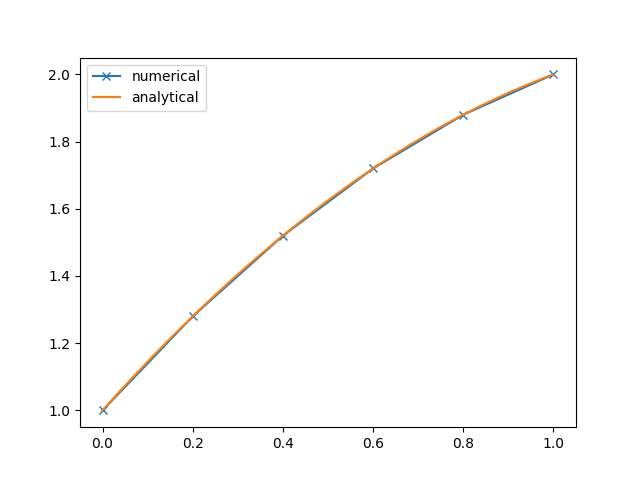
\includegraphics[width=.9\linewidth]{u1sym.png}
      \caption{Numerical and analytical solution of u1}
    \end{subfigure}%
    \begin{subfigure}{.5\textwidth}
      \centering
      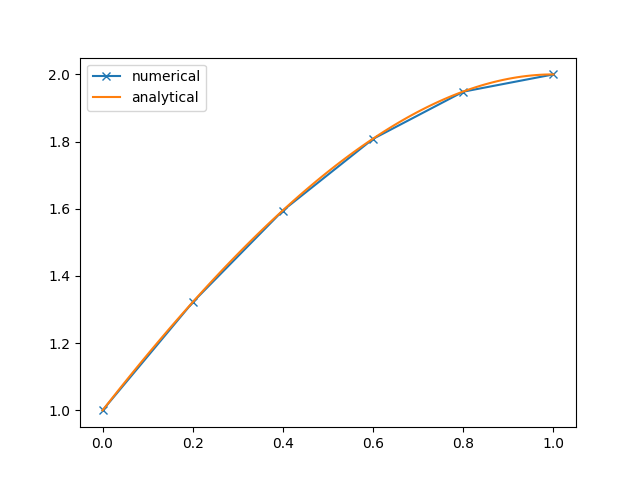
\includegraphics[width=.9\linewidth]{u2sym.png}
      \caption{Numerical and analytical solution of u2}
    \end{subfigure}
    \caption{Comparison of numerical and analytical solutions to the BVP}
\end{figure}
The domain can be refined by decreasing h. This will reduce the global error in the domain. By plotting the global error against the stepsize h, the rate of convergence can be seen. As this plot covers a high range of values, it is bettter to plot it on a double logarithmic plot, this also makes the plot appear linear. In order to understand the rate of convergence a logarithmic function of the form $f(x) = Ch^{\alpha}$. Fitting this function yields $\alpha=1.99$ and $C = 0.0127$. This confirms that the approximation is of second order.
\begin{figure}[H]
    \centering
    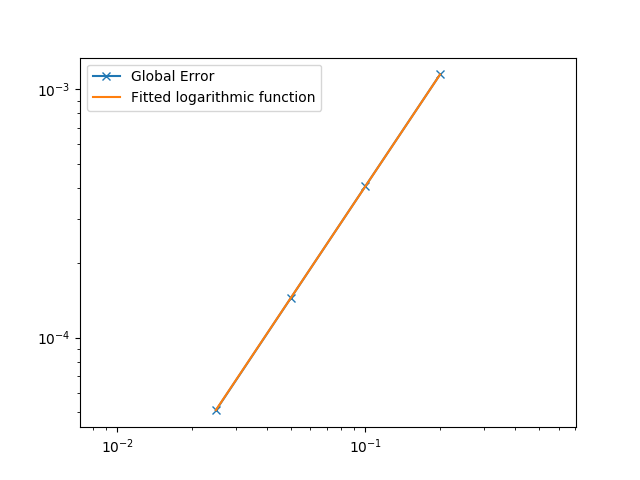
\includegraphics[width=.9\linewidth]{convergence.png}
    \caption{Convergence plot of the BVP}
\end{figure}

\subsection{Asymmetrical Domain}
When considering a domain where one of the inner points has been removed, the discretization of the negative Laplacian changes changes
\begin{figure}[H]
    \centering
    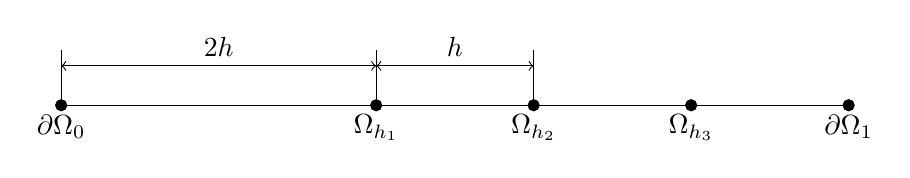
\begin{tikzpicture}
        \foreach \x in {2,...,4} 
            \filldraw (2*\x,5) circle (2pt);

        \filldraw (10,5) circle (2pt);
        \filldraw (0,5) circle (2pt);
        \draw (0,5) node[anchor=north] {$\partial \Omega_0$};

	  \draw (4,5) node[anchor=north] {$\Omega_{h_1}$};
	  \draw (6,5) node[anchor=north] {$\Omega_{h_2}$};
        \draw (8,5) node[anchor=north] {$\Omega_{h_3}$};	
        \draw (10,5) node[anchor=north] {$\partial \Omega_1$};
        \draw (0,5) -- (10,5);
        
      \draw[arrows=<->](4,5.5) -- (6,5.5);
      \draw (4,5) -- (4,5.7);
      \draw (6,5) -- (6,5.7);
      \draw (5,5.5) node[anchor=south] {$h$};
      
      \draw[arrows=<->](4,5.5) -- (0,5.5);
      \draw (0,5) -- (0,5.7);
      \draw (2,5.5) node[anchor=south] {$2h$};
    \end{tikzpicture}
\end{figure}

In order to derive an approximation for the negative Laplacian around $\Omega_{h_1}$, the Taylor series expansions of u at $\partial \Omega_0$ and $\Omega_{h_2}$ are considered.

\begin{equation}
	\partial \Omega_0 = x_{-1},  \Omega_{h_1} = x_0, \Omega_{h_2} = x_1
\end{equation}

\begin{align}
	u(x_{-1}) &= u(x_0) - 2h u'(x_0) + 2h^2u''(x_0)-\frac{4}{3}h^3u'''(x_0) +\mathcal{O}(h^4)\\
	u(x_{0}) &= u(x_0)\\
	u(x_{1}) &= u(x_0) +h u'(x_0) + \frac{1}{2}h^2u''(x_0)+\frac{1}{6}h^3u'''(x_0)+\mathcal{O}(h^4)
\end{align}

With these expansion $-u''(x_{0})$ can be approximated by $\frac{1}{h^2}(-\frac{1}{3}u(x_{-1})+u(x_{0})-\frac{2}{3}u(x_{1}))$. 
\begin{equation}
-u''(x_{0})=\frac{-\frac{1}{3} u(x_{-1}) + u(x_{0}) - \frac{2}{3} u(x_{1})}{h^2}+\mathcal{O}(h)
\end{equation}
Solving the Problem on the asymmetrical domain for $h=0.2$ yields the following results. It can be seen that the global error for $u_1$ is zero, as the discrete solutions lie on the exact solution. This is the same superconvergence that can be seen on the symmetrical domain.
\begin{table}[H]
    \centering
    \begin{tabular}{c|c|c|c|c}
            & $u_1$ numerical & $u_1$ analytical & $u_2$ numerical & $u_2$ analytical \\ \hline
        0.4 & 1.52 & 1.52 & 1.6013 & 1.5954 \\ \hline
        0.6 & 1.72 & 1.72 & 1.8125 & 1.8089 \\ \hline
        0.8 & 1.88 & 1.88 & 1.9508 & 1.9490 \\ \hline
        L2h Error& $0$ & N/A &0.00708 & N/A
    \end{tabular}
\end{table}

\begin{figure}[H]
    \begin{subfigure}{.5\textwidth}
      \centering
      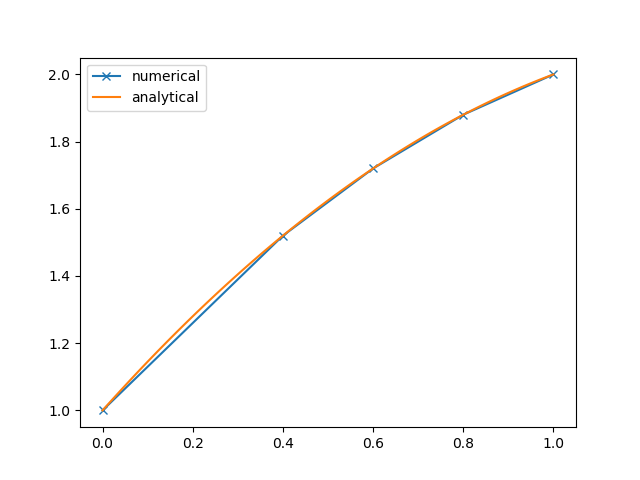
\includegraphics[width=.9\linewidth]{u1asym.png}
      \caption{Numerical and analytical solution of u1}
    \end{subfigure}%
    \begin{subfigure}{.5\textwidth}
      \centering
      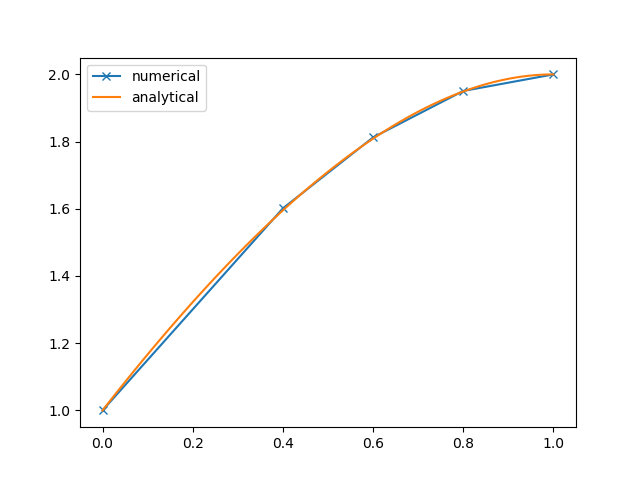
\includegraphics[width=.9\linewidth]{u2asym.png}
      \caption{Numerical and analytical solution of u2}
    \end{subfigure}
    \caption{Comparison of numerical and analytical solutions to the BVP on an asymmetrical domain}
\end{figure}
A convergence analysis can also be performed for this asymmetrical domain. Fitting an exponential of the form $Ch^{\alpha}$ it is found that $\alpha=2.936$ and $C=0.357$. Comparing this to the symmetrical domain, it can be seen that the convergence is faster for this magnitude of h, however the global error is  approximately one magnitude bigger for big $h$. It can be expected that the rate of convergence reduces for further refinements of $h$.

\begin{figure}[H]
	\centering
	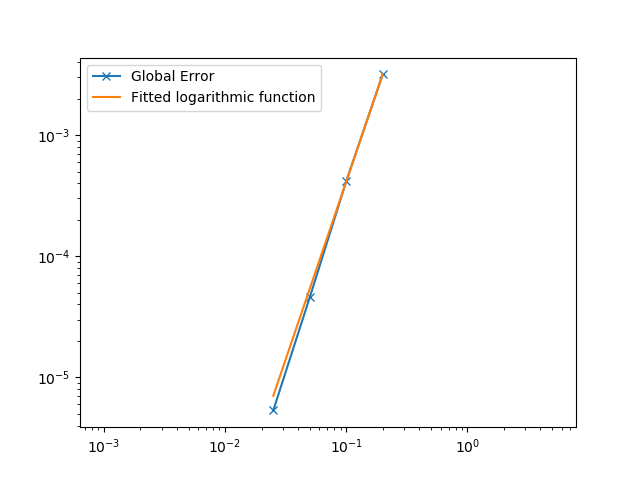
\includegraphics[width=.9\linewidth]{convergenceasym.png}
	\caption{Convergence plot on the asymetrical domain}
\end{figure}

\section{2D boundary value problem}
In this section the following BVP will be solved.
\begin{equation}
\begin{aligned}-\Delta u &=f, \quad(x, y) \in \Omega=(0,2) \times(0,1) \\ u(x, y) &=\sin (2 \pi y), \quad x=0, y \in[0,1] \\ u(x, y) &=\sin (2 \pi y), \quad x=2, y \in[0,1] \\ u(x, y) &=\sin (0.5 \pi x), \quad x \in[0,2], y=0 \\ u(x, y) &=0, \quad x \in[0,2], y=1 \\ f(x, y) &=20 \sin (\pi y) \sin (1.5 \pi x+\pi), \quad(x, y) \in \bar{\Omega} \end{aligned}
\end{equation}

First a finite difference discretization is derived for a single point.

\begin{figure}[H]
	\centering
	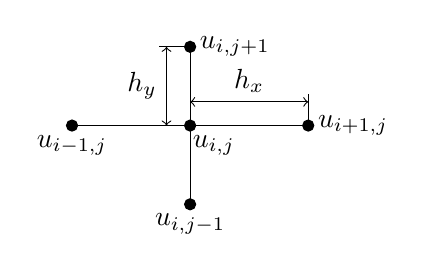
\begin{tikzpicture}
		\filldraw (0,0) circle (2pt);
		\draw (0.3,0) node[anchor=north] {$u_{i,j}$};
		
		\filldraw (-1.5,0) circle (2pt);
		\draw (-1.5,0) node[anchor=north] {$u_{i-1,j}$};
		
		\filldraw (1.5,0) circle (2pt);
		\draw (1.5,0) node[anchor=west] {$u_{i+1,j}$};
		
		\filldraw (0,-1) circle (2pt);
		\draw (0,-1) node[anchor=north] {$u_{i,j-1}$};
		
		\filldraw (0,1) circle (2pt);
		\draw (0,1) node[anchor=west] {$u_{i,j+1}$};
		
		\draw (-1.5,0) -- (1.5,0);
		\draw (0,-1) -- (0,1);
		
		\draw[arrows=<->](1.5,0.3) -- (0,0.3);
		\draw (1.5,0) -- (1.5,0.4);
		\draw (0.75,0.3) node[anchor=south] {$h_x$};
		
		\draw[arrows=<->](-0.3, 0) -- (-0.3,1);
		\draw (0,1) -- (-0.4,1);
		\draw (-0.3,0.5) node[anchor=east] {$h_y$};
	\end{tikzpicture}
	\caption{Stencil used for the discretization}
\end{figure}
Similarly to the previous BVP, the negative second derivative of u is given by.
\begin{align}
	-\frac{\partial^2 u}{\partial x^2} &= \frac{-u_{i-1,j}+2u_{i,j}-u_{i+1,j}}{h_x^2} + \mathcal{O}(h_x^2)\\
	-\frac{\partial^2 u}{\partial y^2} &= \frac{-u_{i,j-1}+2u_{i,j}-u_{i,j+1}}{h_y^2} + \mathcal{O}(h_y^2)
\end{align}
As $-\Delta u=\mathcal{L}u = -\frac{\partial^2u}{\partial x^2} - \frac{\partial^2u}{\partial x^2}$.
\begin{equation}
	-\Delta u \approx \frac{-u_{i-1,j}+2u_{i,j}-u_{i+1,j}}{h_x^2} + \frac{-u_{i,j-1}+2u_{i,j}-u_{i,j+1}}{h_y^2}+\mathcal{O}(h_x^2+h_y^2)
\end{equation}

In order to reduce the computational effort of building the linear system by hand, this idea is extended to an arbitrarily large grid.

Let $L$ be a discretized version of the negative Laplacian acting on a lexicographig vector of a 2 dimensional rectangular evenly spaced grid with $n_x$ and $n_y$ inner points.
\begin{align}
    L\mathbf{u} &\approx \mathcal{L} u\\
\end{align}

As $L$ is a linear operator, we can split it up into 2 seperate operators. Where $D_x'$ and $D_y'$ are the unknown versions of the discretized negative second derivative operators.

\begin{equation}
    L = D_x' + D_y'
\end{equation}

Lets consider a Matrix $M$.
\begin{equation}
    M = \begin{bmatrix}
        u_{1,1} & u_{1,2} & \dots & u_{1,n_y} \\
        u_{2,1} & u_{2,2} & \dots & u_{2,n_y} \\
        \vdots & \vdots & \ddots & \vdots \\
        u_{n_x,1} & u_{n_x,2} & \dots & u_{n_x,n_y}
    \end{bmatrix}
\end{equation}

Lets consider the discrete 1D versions of the Laplacian as $D_x$ and $D_y$, with sizes $n_x \times n_x$ and $n_y \times n_y$ respectively.
Let $M_x$ and $M_y$ be $n_x\times n_y$ matrices containing approximated negative second derivatives of $\mathbf{u}$ order similarly as in $M$. It than can easily proven that.
\begin{align}
    D_x M = M_x \\
    M D_y = M_y
\end{align}
Lets introduce $\operatorname{vec}(A)=\left[a_{1,1}, \ldots, a_{m, 1}, a_{1,2}, \ldots, a_{m, 2}, \ldots, a_{1, n}, \ldots, a_{m, n}\right]^{\mathrm{T}}$ as the vectorization of a Matrix. With this Operators, the following properties emerge.
\begin{align}
    \operatorname{vec}(M) &= \mathbf{u} \\
    \operatorname{vec}(M_x) + \operatorname{vec}(M_y) &= L\mathbf{u}
\end{align}
Using $\operatorname{vec}(A B)=\left(I_{m} \otimes A\right) \operatorname{vec}(B)=\left(B^{\mathrm{T}} \otimes I_{k}\right) \operatorname{vec}(A)$ and $D_y^{\mathrm{T}} = D_y$. Where $\otimes$ denotes the Kronecker product.
\begin{align}
    \operatorname{vec}(D_x M) = (I_{n_y} \otimes D_x)\operatorname{vec}(M) = \operatorname{vec}(M_x)\\
    \operatorname{vec}(M D_y) = (D_y \otimes I_{n_x})\operatorname{vec}(M) = \operatorname{vec}(M_y)
\end{align} 
As $\operatorname{vec}(M) = \mathbf{u}$, $D_x' \mathbf{u} = \operatorname{vec}(M_x)$ and $D_y' \mathbf{u} = \operatorname{vec}(M_y)$.
\begin{align}
    (I_{n_y} \otimes D_x) = D_x' \\
    (D_y \otimes I_{n_x}) = D_y'
\end{align}
Thus $(I_{n_y} \otimes D_x) + (D_y \otimes I_{n_x}) = L$\par
$D_x$ can be build as $A_x^T A_x$ where $A_x$ where $A_x \in \mathbb{R}^{(n_x+1) \times n_x}$ matrix representing a one sided finite difference approximation for the first derivative.
\begin{equation}
	 A_x = 
     \begin{bmatrix}{1} & {0} & {0} & {0} & {\ldots} & {0} \\ {-1} & {1} & {0} & {0} & {\ldots} & {0} \\ {\vdots} & {} & {} & {} & {} & {\vdots} \\ {0} & {} & {} & {} & {} & {1} \\ {0} & {0} & {0} & {0} & {0} & {-1}\end{bmatrix}
\end{equation}

\begin{equation}
    A_x^T A = \frac{1}{h^2}
    \begin{bmatrix}
        {1}         & {-1}   & {0}   & {0}   & {\ldots}  & {0} \\
        {}        & {1}   & {-1}   & {0}   & {\ldots}  & {0} \\
        {\vdots}    & {}   & {}    & {}    & {}        & {\vdots} \\
        {0}         & {0}    & {0}   & {0}   & {1}       & {-1}
        \end{bmatrix}
    \begin{bmatrix}
    {1} & {0} & {0} & {0} & {\ldots} & {0} \\
    {-1} & {1} & {0} & {0} & {\ldots} & {0} \\
    {\vdots} & {} & {} & {} & {} & {\vdots} \\
    {0} & {} & {} & {} & {} & {1} \\
     {0} & {0} & {0} & {0} & {0} & {-1}
    \end{bmatrix}= 
    \begin{bmatrix}
    	2 & -1 & 0 &  \dots & 0 \\
    	-1 & 2 & -1	&  \dots & 0 \\
    	&  &\ddots&  &  \vdots\\
    	&  &&\ddots&    \vdots\\
    	0&0&0&-1&2\\
    \end{bmatrix}=D_x
\end{equation}


In order to apply the Dirichlet Boundary Conditions, a vector $\mathbf{b}$ has to be added to the right hand side of the System. Let the Boundaries of th domain be denoted by North, West, South and East with their functions $f_N, f_W, f_S, f_E$ respectively. Let $\mathbf{b}_N = \left[f_N(h_x), f_N(h_x*2), \dots, f_N(h_x*n_x)\right]^T$. $\mathbf{b}_W, \mathbf{b}_S \text{ and }  \mathbf{b}_E$ are constructed in a similar way.\par
Let $\mathbf{e}_{m,n}$ denote a unitvector of size m with a 1 in the n\textsuperscript{th} postion.
Then $\mathbf{b} = \frac{1}{h^2}(\mathbf{e}_{n_y,1} \otimes \mathbf{b}_S + \mathbf{e}_{n_y,n_y} \otimes \mathbf{b}_S + \mathbf{b}_W \otimes \mathbf{e}_{n_x,1} + \mathbf{b}_E \otimes \mathbf{e}_{n_x,n_x})$.

Solving $L\mathbf{u} = \mathbf{f}+\mathbf{b}$ with $h=0.02$ yields the following solution.

\begin{figure}[H]
	\begin{subfigure}{.5\textwidth}
		\centering
		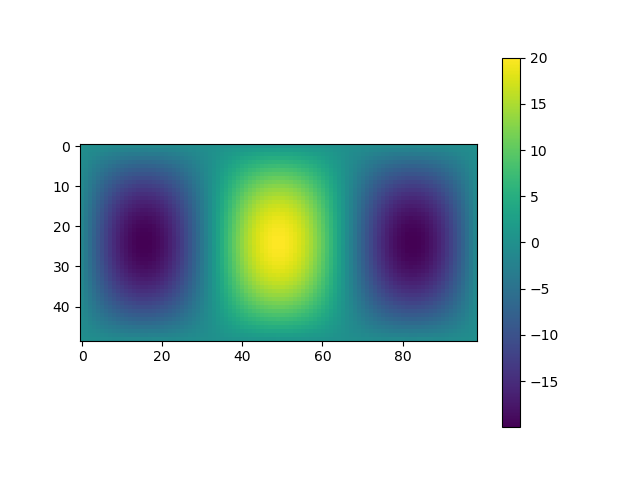
\includegraphics[width=.9\linewidth]{source.png}
		\subcaption{sourcefunction on the domain}
	\end{subfigure}
	\begin{subfigure}{.5\textwidth}
		\centering
		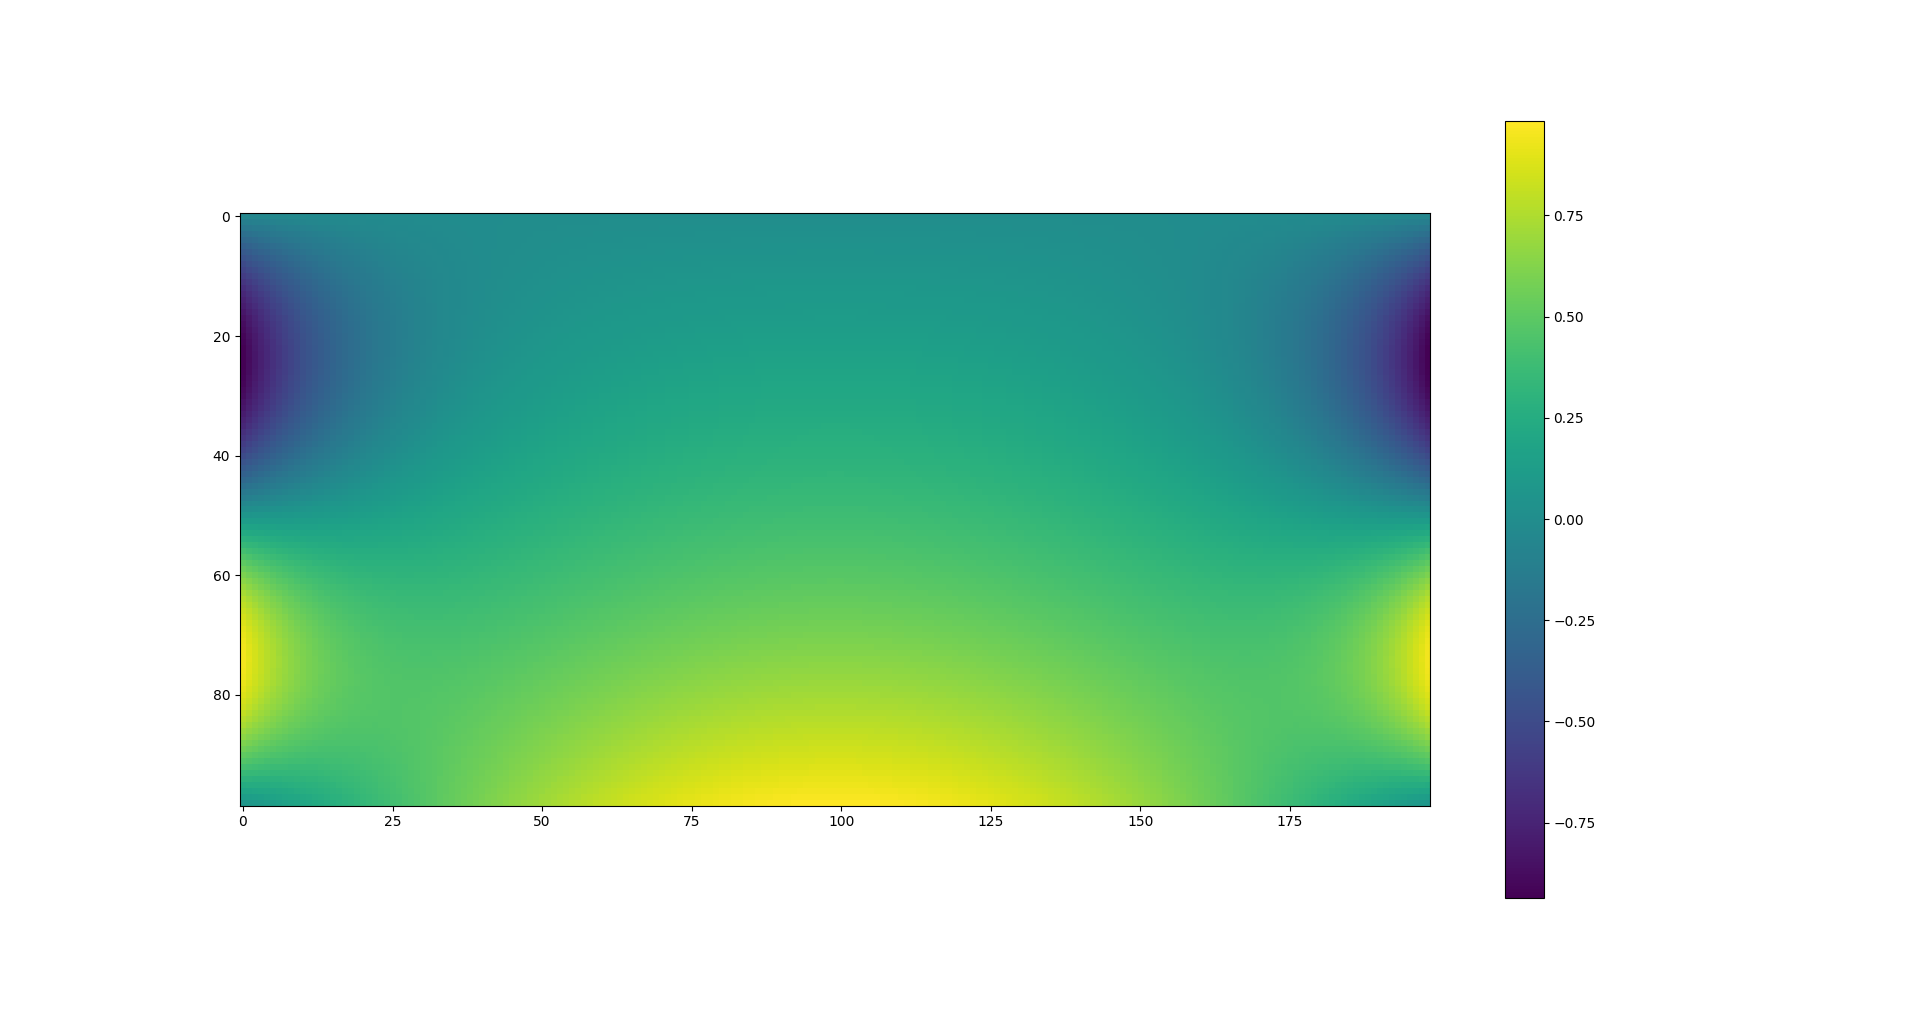
\includegraphics[width=.9\linewidth]{Figure_1.png}
		\subcaption{solution of the BVP on the domain}
	\end{subfigure}
	\caption{Source and Solution of the BVP}
\end{figure}

%\end{multicols}
\end{document}